\documentclass[10pt]{beamer}

\usetheme[progressbar=frametitle]{metropolis}
\usepackage{appendixnumberbeamer}

\usepackage{booktabs}
\usepackage[scale=2]{ccicons}

\usepackage{pgfplots}
\usepgfplotslibrary{dateplot}

\usepackage{xspace}
\newcommand{\themename}{\textbf{\textsc{metropolis}}\xspace}

\usepackage{graphicx}
\graphicspath{ {pics/} }

\usepackage{listings}
\definecolor{mGreen}{rgb}{0,0.6,0}
\definecolor{mGray}{rgb}{0.5,0.5,0.5}
\definecolor{mPurple}{rgb}{0.58,0,0.82}
\definecolor{backgroundColour}{rgb}{0.95,0.95,0.92}

\lstdefinestyle{CStyle}{
    backgroundcolor=\color{backgroundColour},   
    commentstyle=\color{mGreen},
    keywordstyle=\color{magenta},
    numberstyle=\tiny\color{mGray},
    stringstyle=\color{mPurple},
    basicstyle=\footnotesize,
    breakatwhitespace=false,         
    %breaklines=true,                 
    captionpos=b,                    
    keepspaces=true,                 
    %numbers=left,                    
    numbersep=5pt,                  
    showspaces=false,                
    showstringspaces=false,
    showtabs=false,                  
    tabsize=2,
    language=C
}

%----------------------------------------------------------------------------------------
%	TITLE PAGE
%----------------------------------------------------------------------------------------

\title{Netze und Verteilte Systeme}
\subtitle{Programmierprojekt Teil 3}
% \date{\today}
\date{}
\author{Dmitrii Polianskii, Lukas Lamminger}
\institute{Universit\"at Salzburg}
% \titlegraphic{\hfill\includegraphics[height=1.5cm]{logo.pdf}}

\begin{document}

\maketitle

% \begin{frame}{Themen}
%   \setbeamertemplate{section in toc}[sections numbered]
%   \tableofcontents[hideallsubsections]
% \end{frame}

%----------------------------------------------------------------------------------------
%	Einleitung
%----------------------------------------------------------------------------------------

\section{Description}

\begin{frame}[fragile]{Usage TX}
	\begin{block}{C:}
		\hspace*{2mm} \footnotesize 	 ./TX ipAddr portRX packet\_size send\_delay file\_name
	\end{block}

	\begin{block}{java:}
		\hspace*{2mm} \footnotesize 	 java TX ipAddr portRX packet\_size send\_delay file\_name
	\end{block}
		
  \begin{itemize}
  	\footnotesize 	
    \item{\textbf{ipAddr}} - IP address to send datagrams (default: 127.0.0.1)
    \item{\textbf{portRX}} - port to send datagrams (default: 4711)
    \item{\textbf{packet\_size}} - size of a packet in Bytes (default: 1000)
    \item{\textbf{send\_delay}} - delay in microsec between blocks (default: 200)
    \item{\textbf{file\_name}} - name of a file to transmit (default: to\_send.jpg)
  \end{itemize}
\end{frame}

\begin{frame}[fragile]{Usage RX}
	\begin{block}{C:}
		\hspace*{2mm} \footnotesize ./RX portRX
	\end{block}

	\begin{block}{java:}
		\hspace*{2mm} \footnotesize java portRX
	\end{block}
		
  \begin{itemize}
  	\footnotesize 	
    \item{\textbf{portRX}} - port to recieve datagrams (default: 4711)
  \end{itemize}
\end{frame}

\begin{frame}[fragile]{Header structure}

  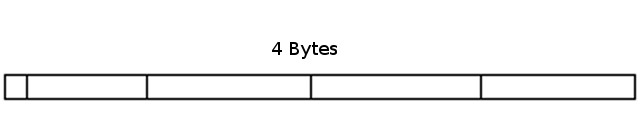
\includegraphics[width=\linewidth]{header}
  \newline
  A header consists of 4 bytes. 
  \newline
  First bit is used to indicate the last packet. 
  \newline
  31 bits left for sequence number

\end{frame}


\begin{frame}[fragile]{TX description}
	\begin{block}{TX description}
		\begin{enumerate}
		\item Read file
		\begin{enumerate}
			\item Read file in buffer
			\item Calculate CRC32 and add to filebytes
			\item Split filebytes in packages
		\end{enumerate}
		\item Initialize UPD Socket
		\item Transmit one packet
		\item Wait for acknowlegment \{DELAY\} microseconds.
		\begin{enumerate}
			\item If a right acknowlegment was recieved -> send next packet.
			\item If all packets were acknowlegment - end transmission. 
		\end{enumerate}
		\end{enumerate}
	\end{block}
\end{frame}




\begin{frame}[fragile]{RX description}
	\begin{block}{RX description}
		\begin{enumerate}
		\item Initialize UPD Socket
		\item Listen for incomming packages
		\begin{enumerate}
			\item Write databits from package in a memory
			\item Send an acknowlegment packet with seq\_num as payload
			\item If last-package-bit was seen, the size of file and Amount of packets can be defined.
			\item If not all of package were recieved, then goto punkt 2.
		\end{enumerate}
		\item Assemble a file
		\item Calculate CRC32 and compare with recieved one.
		\end{enumerate}
	\end{block}
\end{frame}

\section{Tests}


\begin{frame}[fragile]{Tests description}
  \begin{itemize}
  	\footnotesize 	
    \item{} For each set of parameters, the speed measurement is performed 10 times. After that, the average value is calculated
    \item{} The running time and the transfer rate are calculated only for the file transfer phase. Time for initialization and assembly / disassembly of the file is not taken into account.
    \item{} System Characteristics: 
	  \begin{itemize}
	    \item{} OS: Ubuntu 18.04 64-bit
	    \item{} Processor: AMD Ryzen @ 3.50GHz x 4
	    \item{} Memory: 8GB 
	  \end{itemize}
    \item{} Secont System for WLAN tests: 
	  \begin{itemize}
	    \item{} OS: Ubuntu 16.04 64-bit
	    \item{} Processor: Pentium T4200 @ 2.00GHz x 2
	    \item{} Memory: 4GB 
	  \end{itemize}
  \end{itemize}
\end{frame}


\section{Tests: C to C}

\begin{frame}[fragile]{TX.c to RX.c}
	\begin{block}{TX.c to RX.c: Manipulate delays}
	\begin{table}[]
	\scriptsize 
	\centering
		\begin{table}[]
			\centering
			\label{my-label}
			\begin{tabular}{@{}llllll@{}}
				\toprule
				File size & \begin{tabular}[c]{@{}l@{}}Packet size \\ (Bytes)\end{tabular} & \begin{tabular}[c]{@{}l@{}}Delay \\ (microseconds)\end{tabular} & \begin{tabular}[c]{@{}l@{}}Elapsed time \\ (s)\end{tabular} & \begin{tabular}[c]{@{}l@{}}Speed \\ (Mbps)\end{tabular} \\ 
				\midrule
				100Kb & 1000 & 200 & 0.003 & 258,98 \\ 
				\midrule
				100Kb & 1000 & 50 & 0.003 & 254,92 \\ 
				\midrule
				100Kb & 1000 & 10 & 0,004 & 223,3 \\ 
				\midrule
				1Mb & 1000 & 200 & 0,025 & 322,0 \\ 
				\midrule
				1Mb & 1000 & 50 & 0,024 & 332,0 \\ 
				\midrule
				1Mb & 1000 & 10 & 0,023 & 347,8 \\ 
				\midrule
				10Mb & 1000 & 200 & 0,207 & 386,4 \\ 
				\midrule
				10Mb & 1000 & 50 & 0,226 & 352,9 \\ 
				\midrule
				10Mb & 1000 & 10 & 0,314 & 254,3 \\ 
				\bottomrule
			\end{tabular}	
		\end{table}
	\end{table}

	\end{block}
\end{frame}

\begin{frame}[fragile]{TX.c to RX.c}
	\begin{block}{TX.c to RX.c: Manipulate with size of packet}
	\begin{table}[]
	\scriptsize 
	\centering
		\begin{table}[]
			\centering
			\label{my-label}
			\begin{tabular}{@{}llllll@{}}
				\toprule
				File size & \begin{tabular}[c]{@{}l@{}}Packet size \\ (Bytes)\end{tabular} & \begin{tabular}[c]{@{}l@{}}Delay \\ (microseconds)\end{tabular} & \begin{tabular}[c]{@{}l@{}}Elapsed time \\ (s)\end{tabular} & \begin{tabular}[c]{@{}l@{}}Speed \\ (Mbps)\end{tabular} \\ 
				\midrule
				100Kb & 1000 & 50 & 0.003 & 254,92 \\ 
				\midrule
				100Kb & 10000 & 50 & 0.001 & 786,1 \\
				\midrule
				1Mb & 1000 & 50 & 0,024 & 332,0 \\ 
				\midrule
				1Mb & 10000 & 50 & 0,007 & 1198,0 \\ 
				\midrule
				1Mb & 65000 & 50 & 0,004 & 2407,6 \\ 
				\midrule
				10Mb & 1000 & 50 & 0,226 & 352,9 \\ 
				\midrule
				10Mb & 10000 & 50 & 0,058 & 1378,32 \\ 
				\midrule
				10Mb & 65000 & 50 & 0,034 & 2298,6 \\ 
				\bottomrule
			\end{tabular}	
		\end{table}
	\end{table}

	\end{block}
\end{frame}

\begin{frame}[fragile]{TX.c to RX.c}
	\begin{block}{TX.c to RX.c: WLAN tests}
	\begin{table}[]
	\scriptsize 
	\centering
		\begin{table}[]
			\centering
			\label{my-label}
			\begin{tabular}{@{}llllll@{}}
				\toprule
				File size & \begin{tabular}[c]{@{}l@{}}Packet size \\ (Bytes)\end{tabular} & \begin{tabular}[c]{@{}l@{}}Delay \\ (microseconds)\end{tabular} & \begin{tabular}[c]{@{}l@{}}Elapsed time \\ (s)\end{tabular} & \begin{tabular}[c]{@{}l@{}}Speed \\ (Mbps)\end{tabular} \\ 
				\midrule
				100Kb & 1000 & 1000 & 0.310 & 2,7 \\ 
				\midrule
				100Kb & 1000 & 2000 & 0.211 & 3.8 \\
				\midrule
				100Kb & 10000 & 5000 & 0.108 & 8.26 \\
				\midrule
				100Kb & 10000 & 20000 & 0.068 & 13.87 \\
				\midrule
				1Mb & 1000 & 2000 & 2.191 & 4.0 \\ 
				\midrule
				1Mb & 10000 & 10000 & 0,651 & 13.4 \\ 
				\midrule
				1Mb & 50000 & 50000 & 0,571 & 15.3 \\ 
				\midrule
				10Mb & 1000 & 2000 & 24,721 & 3,4 \\ 
				\midrule
				10Mb & 10000 & 10000 & 7.14 & 11.8 \\ 
				\midrule
				10Mb & 50000 & 50000 & 4.97 & 16.9 \\ 
				\bottomrule
			\end{tabular}	
		\end{table}
	\end{table}

	\end{block}
\end{frame}

\section{Tests: C to Java}

\begin{frame}[fragile]{TX.c to RX.java}
	\begin{block}{TX.c to RX.java: Manipulate delays}
	\begin{table}[]
	\scriptsize 
	\centering
		\begin{table}[]
			\centering
			\label{my-label}
			\begin{tabular}{@{}llllll@{}}
				\toprule
				File size & \begin{tabular}[c]{@{}l@{}}Packet size \\ (Bytes)\end{tabular} & \begin{tabular}[c]{@{}l@{}}Delay \\ (microseconds)\end{tabular} & \begin{tabular}[c]{@{}l@{}}Elapsed time \\ (s)\end{tabular} & \begin{tabular}[c]{@{}l@{}}Speed \\ (Mbps)\end{tabular} \\ 
				\midrule
				100Kb & 1000 & 200 & 0,035 & 28.3 \\ 
				\midrule
				100Kb & 1000 & 1000 & 0,029 & 33.7 \\ 
				\midrule
				100Kb & 1000 & 5000 & 0,030 & 32.1 \\ 
				\midrule
				1Mb & 1000 & 200 & 0,086 & 109.0 \\ 
				\midrule
				1Mb & 1000 & 1000 & 0,084 & 109.1 \\ 
				\midrule
				1Mb & 1000 & 5000 & 0,089 & 104.4 \\ 
				\midrule
				10Mb & 1000 & 200 & 0.511 & 165.2 \\ 
				\midrule
				10Mb & 1000 & 1000 & 0.552 & 153.9 \\ 
				\midrule
				10Mb & 1000 & 5000 & 0.515 & 165.0 \\ 
				\bottomrule
			\end{tabular}	
		\end{table}
	\end{table}

	\end{block}
\end{frame}

\begin{frame}[fragile]{TX.c to RX.java}
	\begin{block}{TX.c to RX.java: Manipulate with size of packet}
	\begin{table}[]
	\scriptsize 
	\centering
		\begin{table}[]
			\centering
			\label{my-label}
			\begin{tabular}{@{}llllll@{}}
				\toprule
				File size & \begin{tabular}[c]{@{}l@{}}Packet size \\ (Bytes)\end{tabular} & \begin{tabular}[c]{@{}l@{}}Block size \\ (packets)\end{tabular} & \begin{tabular}[c]{@{}l@{}}Delay \\ (microseconds)\end{tabular} & \begin{tabular}[c]{@{}l@{}}Elapsed time \\ (s)\end{tabular} & \begin{tabular}[c]{@{}l@{}}Speed \\ (Mbps)\end{tabular} \\ 
				\midrule
				100Kb & 1000 & 200 & 0,035 & 28.3 \\ 
				\midrule
				100Kb & 10000 & 200 & 0,021 & 37.4 \\
				\midrule
				1Mb & 1000 & 200 & 0,086 & 109.0 \\ 
				\midrule
				1Mb & 10000 & 200 & 0,061 & 146.4 \\ 
				\midrule
				1Mb & 65000 & 200 & 0,051 & 175.9 \\ 
				\midrule
				10Mb & 1000 & 200 & 0.511 & 165.2 \\ 
				\midrule
				10Mb & 10000 & 200 & 0.301 & 277.6 \\ 
				\midrule
				10Mb & 65000 & 200 & 0.258 & 341.6 \\ 
				\bottomrule
			\end{tabular}	
		\end{table}
	\end{table}

	\end{block}
\end{frame}

\begin{frame}[fragile]{TX.c to RX.java}
	\begin{block}{TX.c to RX.c: WLAN tests}
	\begin{table}[]
	\scriptsize 
	\centering
		\begin{table}[]
			\centering
			\label{my-label}
			\begin{tabular}{@{}llllll@{}}
				\toprule
				File size & \begin{tabular}[c]{@{}l@{}}Packet size \\ (Bytes)\end{tabular} & \begin{tabular}[c]{@{}l@{}}Delay \\ (microseconds)\end{tabular} & \begin{tabular}[c]{@{}l@{}}Elapsed time \\ (s)\end{tabular} & \begin{tabular}[c]{@{}l@{}}Speed \\ (Mbps)\end{tabular} \\ 
				\midrule
				100Kb & 1000 & 1000 & 0.310 & 2,7 \\ 
				\midrule
				100Kb & 1000 & 2000 & 0.211 & 3.8 \\
				\midrule
				100Kb & 10000 & 5000 & 0.108 & 8.26 \\
				\midrule
				100Kb & 10000 & 20000 & 0.068 & 13.87 \\
				\midrule
				1Mb & 1000 & 2000 & 2.191 & 4.0 \\ 
				\midrule
				1Mb & 10000 & 10000 & 0,651 & 13.4 \\ 
				\midrule
				1Mb & 50000 & 50000 & 0,571 & 15.3 \\ 
				\midrule
				10Mb & 1000 & 2000 & 24,721 & 3,4 \\ 
				\midrule
				10Mb & 10000 & 10000 & 7.14 & 11.8 \\ 
				\midrule
				10Mb & 50000 & 50000 & 4.97 & 16.9 \\ 
				\bottomrule
			\end{tabular}	
		\end{table}
	\end{table}

	\end{block}
\end{frame}

\section{Tests: Java to C}

\begin{frame}[fragile]{TX.java to RX.c}
	\begin{block}{TX.java to RX.c: Manipulate delays}
	\begin{table}[]
	\scriptsize 
	\centering
		\begin{table}[]
			\centering
			\label{my-label}
			\begin{tabular}{@{}llllll@{}}
				\toprule
				File size & \begin{tabular}[c]{@{}l@{}}Packet size \\ (Bytes)\end{tabular} & \begin{tabular}[c]{@{}l@{}}Block size \\ (packets)\end{tabular} & \begin{tabular}[c]{@{}l@{}}Delay \\ (microseconds)\end{tabular} & \begin{tabular}[c]{@{}l@{}}Elapsed time \\ (s)\end{tabular} & \begin{tabular}[c]{@{}l@{}}Speed \\ (Mbps)\end{tabular} \\ 
				\midrule
				100Kb & 1000 & 100 & 1000 & 0,081 & 10,13 \\ 
				\midrule
				100Kb & 1000 & 100 & 2000 & 0,080 & 10,14 \\ 
				\midrule
				1Mb & 1000 & 100 & 1000 & 0,404 & 21,9 \\ 
				\midrule
				1Mb & 1000 & 100 & 2000 & 0,448 & 19,7 \\ 
				\midrule
				10Mb & 1000 & 100 & 1000 & 2,120 & 39,6 \\ 
				\midrule
				10Mb & 1000 & 100 & 2000 & 2.151 & 38,8 \\ 
				\midrule
				10Mb & 1000 & 100 & 5000 & 2.548 & 32,7 \\ 
				\bottomrule
			\end{tabular}	
		\end{table}
	\end{table}

	\end{block}
\end{frame}

\begin{frame}[fragile]{TX.java to RX.c}
	\begin{block}{TX.java to RX.c: Manipulate with size of packet}
	\begin{table}[]
	\scriptsize 
	\centering
		\begin{table}[]
			\centering
			\label{my-label}
			\begin{tabular}{@{}llllll@{}}
				\toprule
				File size & \begin{tabular}[c]{@{}l@{}}Packet size \\ (Bytes)\end{tabular} & \begin{tabular}[c]{@{}l@{}}Block size \\ (packets)\end{tabular} & \begin{tabular}[c]{@{}l@{}}Delay \\ (microseconds)\end{tabular} & \begin{tabular}[c]{@{}l@{}}Elapsed time \\ (s)\end{tabular} & \begin{tabular}[c]{@{}l@{}}Speed \\ (Mbps)\end{tabular} \\ 
				\midrule
				100Kb & 1000 & 100 & 1000 & 0,081 & 10,13 \\ 
				\midrule
				100Kb & 10000 & 100 & 1000 & 0,016 & 53,1 \\
				\midrule
				1Mb & 1000 & 100 & 1000 & 0,404 & 21,9 \\ 
				\midrule
				1Mb & 10000 & 100 & 1000 & 0,088 & 99,0 \\ 
				\midrule
				1Mb & 65000 & 100 & 1000 & 0,020 & 376,9 \\ 
				\midrule
				10Mb & 1000 & 100 & 1000 & 2,120 & 39,6 \\ 
				\midrule
				10Mb & 10000 & 100 & 1000 & 0,482 & 183,8 \\ 
				\midrule
				10Mb & 65000 & 100 & 1000 & 0.136 & 635,4 \\ 
				\bottomrule
			\end{tabular}	
		\end{table}
	\end{table}

	\end{block}
\end{frame}

\begin{frame}[fragile]{TX.java to RX.c}
	\begin{block}{TX.java to RX.c: Manipulate with size of block}
	\begin{table}[]
	\scriptsize 
	\centering
		\begin{table}[]
			\centering
			\label{my-label}
			\begin{tabular}{@{}llllll@{}}
				\toprule
				File size & \begin{tabular}[c]{@{}l@{}}Packet size \\ (Bytes)\end{tabular} & \begin{tabular}[c]{@{}l@{}}Block size \\ (packets)\end{tabular} & \begin{tabular}[c]{@{}l@{}}Delay \\ (microseconds)\end{tabular} & \begin{tabular}[c]{@{}l@{}}Elapsed time \\ (s)\end{tabular} & \begin{tabular}[c]{@{}l@{}}Speed \\ (Mbps)\end{tabular} \\ 
				\midrule
				100Kb & 1000 & 100 & 1000 & 0,081 & 10,13 \\ 
				\midrule
				100Kb & 1000 & 500 & 1000 & 0,013 & 54,8 \\ 
				\midrule
				1Mb & 1000 & 50 & 1000 & 0,418 & 20,9 \\ 
				\midrule
				1Mb & 1000 & 100 & 1000 & 0,404 & 21,9 \\ 
				\midrule
				1Mb & 1000 & 500 & 1000 & 0,574 & 6,9 \\ 
				\midrule
				10Mb & 1000 & 50 & 1000 & 2,312 & 36,2 \\ 
				\midrule
				10Mb & 1000 & 100 & 1000 & 2,120 & 39,6 \\ 
				\midrule
				10Mb & 1000 & 500 & 1000 & 3,288 & 26,2 \\ 
				\midrule
				10Mb & 1000 & 2000 & 1000 & 31,190 & 2,8 \\ 
				\bottomrule
			\end{tabular}	
		\end{table}
	\end{table}

	\end{block}
\end{frame}

\begin{frame}[fragile]{TX.java to RX.c}
	\begin{block}{TX.java to RX.c: Best results}
	\begin{table}[]
	\scriptsize 
	\centering
		\begin{table}[]
			\centering
			\label{my-label}
			\begin{tabular}{@{}llllll@{}}
				\toprule
				File size & \begin{tabular}[c]{@{}l@{}}Packet size \\ (Bytes)\end{tabular} & \begin{tabular}[c]{@{}l@{}}Block size \\ (packets)\end{tabular} & \begin{tabular}[c]{@{}l@{}}Delay \\ (microseconds)\end{tabular} & \begin{tabular}[c]{@{}l@{}}Elapsed time \\ (s)\end{tabular} & \begin{tabular}[c]{@{}l@{}}Speed \\ (Mbps)\end{tabular} \\ 
				\midrule
				100Kb & 1000 & 500 & 1000 & 0,013 & 54,8 \\ 
				\midrule
				1Mb & 65000 & 100 & 1000 & 0,020 & 376,9 \\ 
				\midrule
				10Mb & 65000 & 100 & 1000 & 0.136 & 635,4 \\ 
				\bottomrule
			\end{tabular}	
		\end{table}
	\end{table}

	\end{block}
\end{frame}

\section{Tests: Java to Java}

\begin{frame}[fragile]{TX.java to RX.java}
	\begin{block}{TX.java to RX.java: Manipulate delays}
	\begin{table}[]
	\scriptsize 
	\centering
		\begin{table}[]
			\centering
			\label{my-label}
			\begin{tabular}{@{}llllll@{}}
				\toprule
				File size & \begin{tabular}[c]{@{}l@{}}Packet size \\ (Bytes)\end{tabular} & \begin{tabular}[c]{@{}l@{}}Block size \\ (packets)\end{tabular} & \begin{tabular}[c]{@{}l@{}}Delay \\ (microseconds)\end{tabular} & \begin{tabular}[c]{@{}l@{}}Elapsed time \\ (s)\end{tabular} & \begin{tabular}[c]{@{}l@{}}Speed \\ (Mbps)\end{tabular} \\ 
				\midrule
				100Kb & 1000 & 100 & 1000 & 0,169 & 4,9 \\ 
				\midrule
				100Kb & 1000 & 100 & 2000 & 0,218 & 4,3 \\ 
				\midrule
				1Mb & 1000 & 100 & 1000 & 1,022 & 8,7 \\ 
				\midrule
				1Mb & 1000 & 100 & 2000 & 0,900 & 9,7 \\ 
				\midrule
				10Mb & 1000 & 100 & 1000 & 4,142 & 20,3 \\ 
				\midrule
				10Mb & 1000 & 100 & 2000 & 4,148 & 20,2 \\ 
				\bottomrule
			\end{tabular}	
		\end{table}
	\end{table}

	\end{block}
\end{frame}

\begin{frame}[fragile]{TX.java to RX.java}
	\begin{block}{TX.java to RX.java: Manipulate with size of packet}
	\begin{table}[]
	\scriptsize 
	\centering
		\begin{table}[]
			\centering
			\label{my-label}
			\begin{tabular}{@{}llllll@{}}
				\toprule
				File size & \begin{tabular}[c]{@{}l@{}}Packet size \\ (Bytes)\end{tabular} & \begin{tabular}[c]{@{}l@{}}Block size \\ (packets)\end{tabular} & \begin{tabular}[c]{@{}l@{}}Delay \\ (microseconds)\end{tabular} & \begin{tabular}[c]{@{}l@{}}Elapsed time \\ (s)\end{tabular} & \begin{tabular}[c]{@{}l@{}}Speed \\ (Mbps)\end{tabular} \\ 
				\midrule
				100Kb & 1000 & 100 & 1000 & 0,169 & 4,9 \\ 
				\midrule
				100Kb & 10000 & 100 & 1000 & 0,092 & 8,9 \\
				\midrule
				1Mb & 1000 & 100 & 1000 & 1,022 & 8,7 \\ 
				\midrule
				1Mb & 10000 & 100 & 1000 & 0,710 & 13,2 \\ 
				\midrule
				1Mb & 65000 & 100 & 1000 & 0,378 & 23,7 \\ 
				\midrule
				10Mb & 1000 & 100 & 1000 & 4,142 & 20,3 \\ 
				\midrule
				10Mb & 10000 & 100 & 1000 & 2,788 & 31,9 \\ 
				\midrule
				10Mb & 65000 & 100 & 1000 & 1,91 & 77,5 \\ 
				\bottomrule
			\end{tabular}	
		\end{table}
	\end{table}

	\end{block}
\end{frame}

\begin{frame}[fragile]{TX.java to RX.java}
	\begin{block}{TX.java to RX.java: Manipulate with size of block}
	\begin{table}[]
	\scriptsize 
	\centering
		\begin{table}[]
			\centering
			\label{my-label}
			\begin{tabular}{@{}llllll@{}}
				\toprule
				File size & \begin{tabular}[c]{@{}l@{}}Packet size \\ (Bytes)\end{tabular} & \begin{tabular}[c]{@{}l@{}}Block size \\ (packets)\end{tabular} & \begin{tabular}[c]{@{}l@{}}Delay \\ (microseconds)\end{tabular} & \begin{tabular}[c]{@{}l@{}}Elapsed time \\ (s)\end{tabular} & \begin{tabular}[c]{@{}l@{}}Speed \\ (Mbps)\end{tabular} \\ 
				\midrule
				100Kb & 1000 & 100 & 1000 & 0,169 & 4,9 \\ 
				\midrule
				100Kb & 1000 & 500 & 1000 & 0,167 & 4,9 \\ 
				\midrule
				1Mb & 1000 & 50 & 1000 & 1,010 & 8,8 \\ 
				\midrule
				1Mb & 1000 & 100 & 1000 & 1,022 & 8,7 \\ 
				\midrule
				1Mb & 1000 & 500 & 1000 & 1,188 & 7,5 \\ 
				\midrule
				10Mb & 1000 & 50 & 1000 & 3,87 & 21,7 \\ 
				\midrule
				10Mb & 1000 & 100 & 1000 & 4,142 & 20,3 \\ 
				\midrule
				10Mb & 1000 & 500 & 1000 & 6,388 & 13,9 \\ 
				\bottomrule
			\end{tabular}	
		\end{table}
	\end{table}

	\end{block}
\end{frame}

\begin{frame}[fragile]{TX.java to RX.java}
	\begin{block}{TX.java to RX.java: Best results}
	\begin{table}[]
	\scriptsize 
	\centering
		\begin{table}[]
			\centering
			\label{my-label}
			\begin{tabular}{@{}llllll@{}}
				\toprule
				File size & \begin{tabular}[c]{@{}l@{}}Packet size \\ (Bytes)\end{tabular} & \begin{tabular}[c]{@{}l@{}}Block size \\ (packets)\end{tabular} & \begin{tabular}[c]{@{}l@{}}Delay \\ (microseconds)\end{tabular} & \begin{tabular}[c]{@{}l@{}}Elapsed time \\ (s)\end{tabular} & \begin{tabular}[c]{@{}l@{}}Speed \\ (Mbps)\end{tabular} \\ 
				\midrule
				100Kb & 10000 & 100 & 1000 & 0,092 & 8,9 \\
				\midrule
				1Mb & 65000 & 100 & 5000 & 0,346 & 25,4 \\ 
				\midrule
				10Mb & 65000 & 100 & 1000 & 1,91 & 77,5 \\ 
				\bottomrule
			\end{tabular}	
		\end{table}
	\end{table}

	\end{block}
\end{frame}

\section{Compare the best of results}

\begin{frame}[fragile]{Compare}

  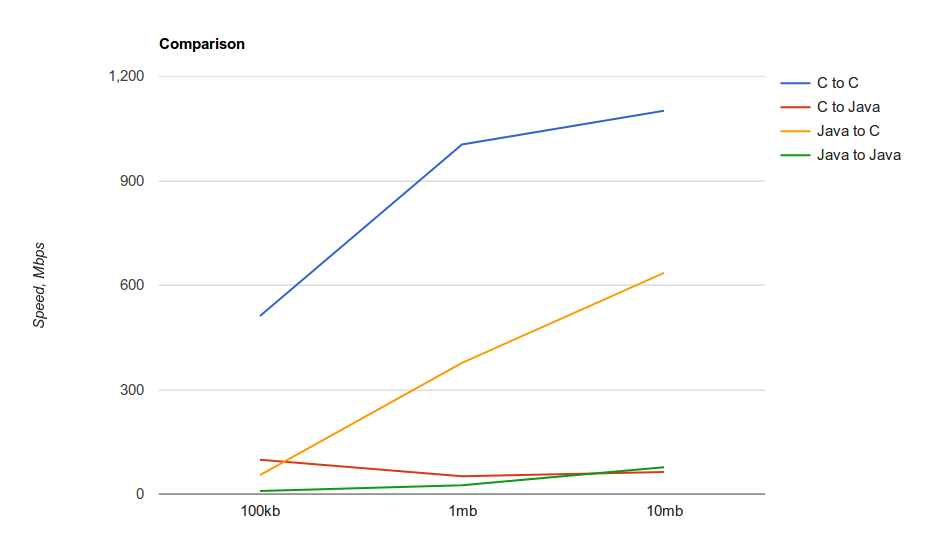
\includegraphics[width=\linewidth]{plot.png}

\end{frame}

\section{WLAN results}

\begin{frame}[fragile]{WLAN c-to-c results}
  \begin{itemize}
  	\footnotesize 	
    \item{} Die Übertragungsrate durch das Shuttle ist um ein Vielfaches niedriger
    \item{} Aufgrund der Tatsache, dass der empfangende Computer viel schwächer ist als das Senden, war es notwendig, den Delay-parameter signifikant zu erhöhen, um akzeptable Geschwindigkeiten zu erreichen
  \end{itemize}
\end{frame}

\end{document}
